\paragraph{Estimating the Regression Coefficients}
A common way to estimate the parameters of a statistical model is to compute
the MLE(Maximum Likelihood Estimation) defined as 
$$\hat{\bm{\theta}} \triangleq \displaystyle \argmax_{\theta} \log\left(
p(\mathcal{D}|\bm{\theta})\right)$$
\begin{align*}
    l(\bm{\theta}) &\triangleq \log\left(p(\mathcal{D}|\bm{\theta})\right)\\
                   &=\su{i=1}{n}\log\left(p(y_{i}|\bm{x_{i}}, \bm{\theta})\right)\\
                   &= \su{i=1}{n}\log\left(
                       \left[\dfrac{1}{2\pi\sigma^{2}}\right]^{\frac{1}{2}}
                       \exp\left(-\dfrac{1}{2\sigma^{2}}\left[y_{i} - \bm{\beta}^{T}
                       \bm{x_{i}}]\right]^{2}\right)\right)\\ 
                   &= \dfrac{1}{2\sigma^{2}}RSS(\bm{\beta}) +
                   \dfrac{n}{2}\log(2\pi\sigma^{2})
\end{align*}
Then the Residual Sum of Squares (RSS) is equal to $\su{i=1}{n}\left(
y_{i}-\beta^{T}x_{i}\right)^{2}$
Instead of maximizing the log-likelihood we can equivalently minimize the Negative Log Likelihood (NLL) 
\begin{center}
    $NLL(\beta) \triangleq l(\beta)$
\end{center}


Considering $\bm{X}$ the $N\times (p+1)$ matrix with each row an input
vector and $y$ be the $N-vector$ of outputs in the training set.
\begin{center}
	$RSS(\beta)=(y-\bm{X}\beta)^{T}(y-\bm{X}\beta)$
\end{center}
Differentiating with respect to $\beta$ we obtain:
$
\begin{cases}
	\dfrac{\partial RSS}{\partial\beta}=-2\bm{X}^{T}(y-\bm{X}\beta)\\
	\dfrac{\partial^{2} RSS}{\partial\beta\partial\beta^{T}}=2\bm{X}^{T}\bm{X}\\
\end{cases}
$\\
Assuming that $\bm{X}$ has full column rank, we set the first 
derivative to 0:\\ $\bm{X}^{T}(y-\bm{X}\beta)=0$ to obtain the unique
solution:

\begin{center}
	\encB{$\hat{\beta}=(\bm{X}^{T}\bm{X})^{-1}\bm{X}^{T}\bm{y}$}
\end{center}
\begin{figure}[H]
\centering
\begin{subfigure}{.5\textwidth}
  \centering
	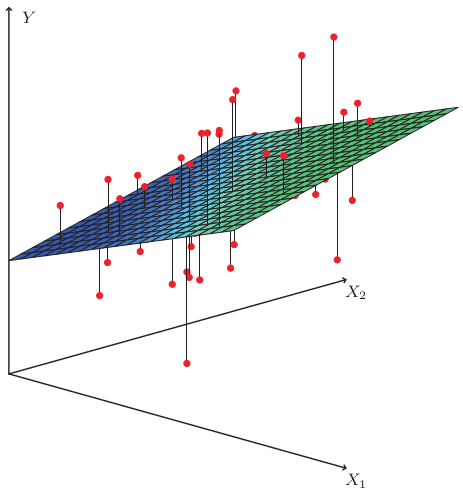
\includegraphics[width=.7\textwidth]{./chap/1chap/2sec/2images/1leastSquaresPlan.png}
  \caption{$n$ observations}
  \label{fig:2.1aLeastSquares}
\end{subfigure}%
\begin{subfigure}{.5\textwidth}
  \centering
	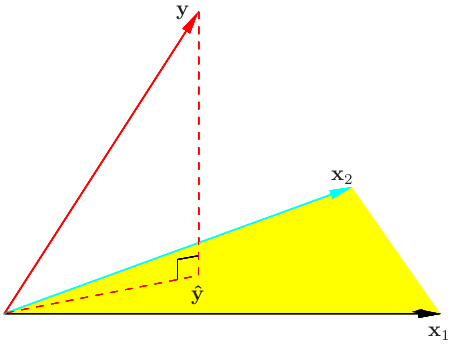
\includegraphics[width=\textwidth]{./chap/1chap/2sec/2images/11projection.png}
\caption{1 observation}
  \label{fig: 2.1bLeastSquares}
\end{subfigure}
  \caption{Least squares for a linear model with $2$ predictors of 
$p$-dimensions.}
\label{fig:test}
\end{figure}

\begin{align*}
\hat{\bm{y}} &=\bm{X}\hat{\beta}\\
	     &=\bm{X}\left(\bm{X}^{T}\bm{X}\right)^{-1}\bm{X}^{T}\bm{y}\\
	     &=\bm{H}\bm{y}
\end{align*}
$\bm{H}$ is called \tB{``hat'' matrix because it puts the hat on $\bm{y}$}.
\paragraph{Hat Matrix}
Residuals can also be expressed as a function of $\bm{H}$,
$\bm{\hat{e}} = \bm{y} - \bm{\hat{y}} = \bm{y} - \bm{Hy} = (\bm{I}-\bm{H})\bm{y}$.
It can be shown that \sB{$\bm{H}$ and $\bm{I}-\bm{H}$ are orthogonal projections}.\\
One can easily show that \tB{$\bm{H}\bm{H} = \bm{H}$} and $\left(\bm{I-H}\right)\left(\bm{I-H}\right)
= \bm{I-H}$

\subparagraph{Range and Kernel of the Hat Matrix}
$rank(\bm{X}) = rank(\bm{X}^{T}\bm{X}) = p^{*}$
\subparagraph{Residual and Fitted Values}
$\bm{H}(\bm{I}-\bm{H}) = \bm{H} -\bm{HH} = 0$, hence $\sP{\bm{\hat{y}}}{\bm{\hat{e}}} = 0$.
\tB{Therefore $\bm{\hat{y}}$ and $\bm{e}$ are orthogonal} in $\mathbb{R}^{n}$.
\subparagraph{Geometric interpretation}
The degrees of freedom associated with \tB{$\bm{\hat{y}}$ and $\bm{\hat{e}}$ can be seen to simply
be the dimensions of the respective vector subspace in which these 2 vectors have been projected}.\\
The vectors $\bm{y}, \bm{\hat{y}}$ and $\bm{\hat{e}}$ determine 3 points in $\mathbb{R}^{n}$ which
form a right-angled triangle, we can see the decomposition of total sum of squares into estimated
sum of squares and residual sum of squares as a special case of \emph{Pythagoras} theorem.
\subparagraph{Further information}
It might happen that the columns of \sB{$\bm{X}$ are not linearly independent, then
$\bm{X}^{T}\bm{X}$ is singular and the least squares coefficients $\hat{\beta}$ are not uniquely 
defined}.\\ 
Knowing that $\V{\bm{A}\bm{y}}=\bm{A}\V{\bm{y}}\bm{A}^{T}$:
\begin{center}
	\encB{$\V{\hat{\beta}}=\left(\bm{X}^{T}\bm{X}\right)^{-1}\sigma^{2}$}
\end{center}
a estimate of $\sigma^{2}$:$\hat{\sigma}^{2} = \dfrac{1}{N-p-1}\su{{i=1}}{N}(y_{i}-\hat{y}_{i})^{2}$ 
The $n-p-1$ rather than $n$ makes $\hat{\sigma}^{2}$ an unbiased
estimate.\\
$
\begin{cases}
\hat{\beta}\hookrightarrow\mathcal{N}\left(\beta, (\bm{X}^{T}\bm{X})^{-1}\sigma^{2}\right)\\
(n-p-1)\hat{\sigma}^{2}\hookrightarrow\sigma^{2}\chi_{n-p-1}^{2}
\end{cases}
$

\paragraph{Convexity}
Functions having a bowl shape with a unique minimum, more precisely:
$$\forall (\bm{\theta}, \bm{\theta'},\lambda) \in \mathcal{S}\times\mathcal{S}\times[0,1],
~ \lambda\bm{\theta} + (1-\lambda)\bm{\theta'} \in \mathcal{S} \Rightarrow \mathcal{S}
\text{ is \textbf{convex}}$$
